\documentclass{beamer}
\setbeamertemplate{footline}[page number]
\date{}
\author{}
\institute{}

%%%%%%% Put these names back in the final version 
%\\Aswathy Rajendra Kurup\\Meenu Ajith}
%\institute{Department of Electrical and Computer Engineering\\The University of New Mexico}
\setbeamercovered{transparent}
\usepackage{setspace}
\usepackage{array}
\usepackage[T1]{fontenc}
\usepackage{graphicx}
\usepackage{amsmath}
\usepackage{amsfonts}
\usepackage{amssymb}
\usepackage{makeidx}
\usefonttheme{serif}
\usepackage{multirow}
\usepackage{booktabs} 
\usepackage{rotating}
\usepackage{color}
\usepackage{float}
\usepackage[latin1]{inputenc}
\usepackage[english]{babel}
\usepackage{amsmath}
\usepackage{amsfonts}
\usepackage{eurosym}
\usepackage{rotating}
\usepackage{multicol}
\usepackage{pythonhighlight}
\usepackage[normalem]{ulem}
\newcommand{\ba}{{\bf a}}
\newcommand{\bb}{{\bf b}}
\newcommand{\bc}{{\bf c}}
\newcommand{\bd}{{\bf d}}
\newcommand{\be}{{\bf e}}
\newcommand{\bbf}{{\bf f}}
\newcommand{\bg}{{\bf g}}
\newcommand{\bh}{{\bf h}}
\newcommand{\bi}{{\bf i}}
\newcommand{\bk}{{\bf k}}
\newcommand{\bl}{{\bf l}}
\newcommand{\bm}{{\bf m}}
\newcommand{\bn}{{\bf n}}
\newcommand{\bo}{{\bf o}}
\newcommand{\bp}{{\bf p}}
\newcommand{\bq}{{\bf q}}
\newcommand{\br}{{\bf r}}
\newcommand{\bs}{{\bf s}}
\newcommand{\bt}{{\bf t}}
\newcommand{\bu}{{\bf u}}
\newcommand{\bv}{{\bf v}}
\newcommand{\bw}{{\bf w}}
\newcommand{\bx}{{\bf x}}
\newcommand{\by}{{\bf y}}
\newcommand{\bz}{{\bf z}}

\newcommand{\bA}{{\bf A}}
\newcommand{\bB}{{\bf B}}
\newcommand{\bC}{{\bf C}}
\newcommand{\bE}{{\bf E}}
\newcommand{\bG}{{\bf G}}
\newcommand{\bH}{{\bf H}}
\newcommand{\bI}{{\bf I}}
\newcommand{\bK}{{\bf K}}
\newcommand{\bL}{{\bf L}}
\newcommand{\bM}{{\bf M}}
\newcommand{\bO}{{\bf O}}
\newcommand{\bQ}{{\bf Q}}
\newcommand{\bR}{{\bf R}}
\newcommand{\bS}{{\bf S}}
\newcommand{\bT}{{\bf T}}
\newcommand{\bV}{{\bf V}}
\newcommand{\bW}{{\bf W}}
\newcommand{\bX}{{\bf X}}
\newcommand{\bY}{{\bf Y}}
\newcommand{\bZ}{{\bf Z}}
\newcommand\uptocnt{\stackrel{\mathclap{\normalfont\mbox{c}}}{\propto}}
\newcommand{\bpt}{{\bf pt}}
\newcommand{\bpl}{{\bf pl}}
\newcommand{\bdp}{{\bf dp}}
\newcommand{\btemp}{{\bf temp}}

\newcommand{\bmu}{{\boldsymbol \mu}}
\newcommand{\bSigma}{{\boldsymbol \Sigma}}
\newcommand{\bsigma}{{\boldsymbol \sigma}}
\newcommand{\bvarPhi}{{\boldsymbol \varPhi}}
\newcommand{\bvarphi}{{\boldsymbol \varphi}}
\newcommand{\bPhi}{{\boldsymbol \Phi}}
\newcommand{\bdelta}{{\boldsymbol \delta}}
\newcommand{\bZero}{{\bf 0}}
\newcommand{\bOne}{{\bf 1}}
\newcommand{\balpha}{{\boldsymbol \alpha}}
\newcommand{\bAlpha}{{\boldsymbol A}}
\newcommand{\btheta}{{\boldsymbol \theta}}

\newcommand{\softmax}{\text{softmax}}
\newcommand{\diag}{\text{diag}}
\newcommand{\sinc}{\mathrm{sinc}}
\newcommand{\argmin}{\mathop{\mathrm{argmin}}}
\newcommand{\infl}{\eta}
\newcommand{\Ind}{\mathrm{I}}
\newcommand{\Real}{\mathbb R}
\newcommand{\Intg}{\mathbb Z}
\newcommand{\Complex}{\mathbb C}
\newcommand{\Natural}{\mathbb N}
\newcommand{\Fourier}[1]{\mathcal{F} \{#1\}}
%\newcommand{\ii}{\mathbbm{i}}
\newcommand{\bphi}{\boldsymbol{\mathit{\phi}}}

\newcommand{\hs}{\hspace{2pt}}
\newcommand{\sign}{\text{sign}}
\author{Manel Mart\'inez-Ram\'on\\Meenu Ajith\\Aswathy Rajendra Kurup}

\usetheme{Madrid}
\usecolortheme{beaver}
\usepackage{tikz}
\usetikzlibrary{fit,arrows,calc,positioning}
\usepackage{listings}
\usepackage{xcolor}
\usepackage{emerald} 
\usepackage[T1]{fontenc} 
\usepackage{verbatim}
\usepackage{graphicx}
\usepackage{epsfig}
\usepackage{psfrag}
\usepackage[english]{babel}
\usepackage{listings}
\usepackage{courier}
\usepackage{color}
 \usepackage{vwcol} 
 \usepackage[english]{babel} % To obtain English text with the blindtext package
\usepackage{blindtext}
\definecolor{codegreen}{rgb}{0,0.6,0}
\definecolor{codegray}{rgb}{0.5,0.5,0.5}
\definecolor{codepurple}{rgb}{0.58,0,0.82}
\definecolor{backcolour}{rgb}{0.95,0.95,0.92}

\lstdefinestyle{mystyle}{
  backgroundcolor=\color{backcolour},   commentstyle=\color{codegreen},
  keywordstyle=\color{magenta},
  numberstyle=\tiny\color{codegray},
  stringstyle=\color{codepurple},
  basicstyle=\ttfamily\footnotesize,
  breakatwhitespace=false,         
  breaklines=true,                 
  captionpos=b,                    
  keepspaces=true,                 
  numbers=left,                    
  numbersep=5pt,                  
  showspaces=false,                
  showstringspaces=false,
  showtabs=false,                  
  tabsize=2
}
\lstset{style=mystyle}

%% Stuff for movies

% %\newcommand{\bt}{{\bf t}}
% \newcommand{\br}{{\bf r}}
% \newcommand{\bs}{{\bf s}}
% \newcommand{\by}{{\bf y}}
% \newcommand{\bz}{{\bf z}}
% \newcommand{\bx}{{\bf x}}
% \newcommand{\bw}{{\bf w}}
% \newcommand{\be}{{\bf e}}
% \newcommand{\bbf}{{\bf f}}
% \newcommand{\bb}{{\bf b}}
% \newcommand{\bd}{{\bf d}}
% \newcommand{\bA}{{\bf A}}
% \newcommand{\bB}{{\bf B}}
% \newcommand{\bL}{{\bf L}}
% \newcommand{\bM}{{\bf M}}

% \newcommand{\bC}{{\bf C}}
% \newcommand{\bI}{{\bf I}}
% \newcommand{\bK}{{\bf K}}
% \newcommand{\bk}{{\bf k}}
% \newcommand{\bT}{{\bf T}}
% \newcommand{\bV}{{\bf V}}
% \newcommand{\bW}{{\bf W}}
% \newcommand{\bX}{{\bf X}}
% \newcommand{\bY}{{\bf Y}}
% \newcommand{\bZ}{{\bf Z}}
% \newcommand{\bm}{{\bf m}}
% \newcommand{\bpt}{{\bf pt}}
% \newcommand{\bpl}{{\bf pl}}
% \newcommand{\bdp}{{\bf dp}}
% \newcommand{\btemp}{{\bf temp}}
% \newcommand{\bl}{{\bf l}}
% \newcommand{\bu}{{\bf u}}
% \newcommand{\bmu}{{\boldsymbol \mu}}
% \newcommand{\bSigma}{{\boldsymbol \Sigma}}
% \newcommand{\bLambda}{{\boldsymbol \Lambda}}

% \newcommand{\bsigma}{{\boldsymbol \sigma}}
% \newcommand{\bvarphi}{{\boldsymbol \varPhi}}
% \newcommand{\btheta}{{\boldsymbol \theta}}
% \newcommand{\bZero}{{\bf 0}}
% \newcommand{\balpha}{{\boldsymbol \alpha}}
% \newcommand{\bpi}{{\boldsymbol \pi}}
% \newcommand{\bxi}{{\boldsymbol \xi}}
% \newcommand{\bdelta}{{\boldsymbol \delta}}
\lstset{
	language=Python,
	basicstyle=\footnotesize\ttfamily\color{black},
	commentstyle = \footnotesize\ttfamily\color{red},
	keywordstyle=\footnotesize\ttfamily\color{blue},
	stringstyle=\footnotesize\ttfamily\color{black},
%	columns=fixed,
%	numbers=left,    
	numberstyle=\tiny,
	stepnumber=1,
	numbersep=5pt,
	tabsize=1,
	extendedchars=true,
	breaklines=true,            
	frame=b,         
	showspaces=false,
	showtabs=true,
	xleftmargin=6pt,
	framexleftmargin=6pt,
	framexrightmargin=2pt,
	framexbottommargin=4pt,
	showstringspaces=false      
}

\lstloadlanguages{
         Python
}

%\graphicspath{ {./images/} }  % Figures path - used in graphicx

%\selectcolormodel{cmyk}

\mode<presentation>

\newcommand{\dred}{darkred!90!black}
\newcommand{\written}{\ECFJD\textcolor{cyan!50!white}}
\newcommand{\hlight}{\textcolor{\dred}}
\newcommand{\Ex}{\textcolor{\dred}{Ex. }}

% remove navigation symbols in full screen mode
\setbeamertemplate{navigation symbols}{}  
\setbeamertemplate{blocks}[rounded][shadow=false]
\setbeamercolor{note page}{fg=black}

\setbeamercolor{title}{fg=\dred}
\setbeamercolor{frametitle}{fg=white}
\setbeamercolor{frametitle}{bg=\dred}
\setbeamercolor{structure}{fg=black,bg=white}
\setbeamercolor{background canvas}{bg=white,fg=black}
\setbeamercolor{normal text}{fg=black,bg=white}
\setbeamercolor{item}{fg=red!80!black,bg=white!}
\addtobeamertemplate{block begin}{\setbeamercolor{block title}{fg=white,bg=\dred}
\setbeamercolor{block body}{fg=white,bg=gray}}{}


\title[5. Recurrent neural networks]{5. Sequence modeling with recurrent neural networks}
\subtitle{5.2a. Training an RNN. Recursive gradients}

\addtobeamertemplate{frametitle}{}


\begin{document}
\maketitle

\begin{frame}{RNN training}{The cost function}
\begin{itemize}
\item Assume an RNN designed to classify among $K$ classes \item A training sequence $\bx_t \in \mathbb{R}^D$, $\by_t \in \mathbb{R}^K$, $1 \leq t \leq T$ is available.
\item We must then maximize the cross entropy between the labels and the outputs or, equivalently, the output likelihood: 
\begin{equation}\label{eq:RNN_cost}
    J_{ML}(\btheta,\bX,\bY)=- \sum_{t=1}^T \ell(\bx_t) =-\sum_{t=1}^T\sum_{k=0}^{K-1} y_{k,t} \log \softmax\left(z^{(o)}_{k,t}\right)
\end{equation}
 where
 \item $\bX = \left[\bx_1 \cdots \bx_T \right]$ and $\bY =\left[\by_1 \cdots \by_T\right]$.
\item  $\btheta = \{\bW_{hx}, \bW_{hh}, \bW_{oh}\}$ contains all trainable parameters. 
\end{itemize}
\end{frame}

\begin{frame}{RNN training}{The Jacobian with respect to $\bh_t$}
\begin{itemize}
\item We  must consider that the hidden state $\bh_t$ at every instant depends on the states $\bh_{t'}$, $t'<t$. \item During the backpropagation  $\nabla_{\bh_t}J_{ML}$ appears. For   $t=T$,
\begin{equation}\label{eq:grad_J_h_T}
    \nabla_{\bh_T}J_{ML} = \frac{\delta \bz^{(o)}_T}{\delta\bh_T} \nabla_{\bz^{(o)}_T}J_{ML}
\end{equation}
where $ \nabla_{\bz^{(o)}_T}J_{ML}$ is the output error: 
\begin{equation}
    \frac{dJ_{ML}}{d z^{(o)}_{k,T}} = 
    \frac{dJ_{ML}}{d o_{k,T}} \frac{o_{k,t}}{d z^{(o)}_{k,T}}  =\frac{dJ_{ML}}{d o_{k,T}} o'_{k,T} =\delta_{k,T}
\end{equation}
 \item Since the output of the RNN is a softmax, $\bdelta_{t} =  \softmax(\bz^{(o)}_{t}) - \by_{t}$
\end{itemize}
\end{frame}

\begin{frame}{RNN training}{The Jacobian with respect to $\bh_t$}
\begin{itemize}
    \item For $t<T$, the cost function in Eq. \eqref{eq:RNN_cost} contains $\bh_t$ in element $\ell(\bx_t)$ and in the next one, $\ell(\bx_{t+1})$ since
\begin{equation}
    \bh_{t+1}=\tanh\left(\bz^{(x)}_{t+1}\right)=\tanh\left(\bW_{hx}^\top\bx_{t+1} + \bW_{hh}^\top\bh_{t}+\bb_{h}\right)
\end{equation}


\item Jacobian $\frac{\delta \bh_{t+1}}{\delta \bh_t} $ will appear in the chain rule, with elements $\frac{\delta h_{j,t+1}}{\delta h_{i,t}}$. By applying the chain rule of calculus to them
\begin{equation}\label{eq:deriv_h_jtau}
    \frac{\delta h_{j,t+1}}{\delta h_{i,t}} = \frac{\delta h_{j,t+1}}{\delta z^{(x)}_{j,t+1}} \frac{\delta z^{(x)}_{j,t+1}}{\delta h_{i,t}} = \frac{\delta h_{j,t+1}}{\delta z^{(x)}_{j,t+1}} \frac{\delta \bw_{j,hh}^\top \bh_{t}}{\delta h_{i,t}}
\end{equation}

\end{itemize}

\end{frame}

\begin{frame}{RNN training}{The Jacobian with respect to $\bh_t$}
\begin{itemize}

\item The first derivative of the right side of expression \eqref{eq:deriv_h_jtau} is the derivative of the hyperbolic tangent. The second derivative is parameter $w_{i,j,hh}$. 
\item Therefore
\begin{equation}\label{eq:deriv_h_jtau_result}
    \frac{\delta h_{j,t+1}}{\delta h_{i,t}} = w_{i,j,hh}\text{tanh}'\left(z^{(x)}_{j,t+1 }\right)
\end{equation}
\item Thus, Jacobian $\frac{\delta\bh_{t+1}}{\delta\bh_{t}}$ is 
\begin{equation}\label{eq:jacobian_h}
  \frac{\delta\bh_{t+1}}{\delta\bh_{t}} = \bW_{hh} \text{diag}\left(\text{tanh}'\left(\bz^{(x)}_{t+1 }\right)\right) 
\end{equation}
\end{itemize}
\end{frame}
\begin{frame}{RNN training}{The Jacobian with respect to $\bh_t$}
\begin{itemize}
    \item  With all these elements, the gradient of the cost function with respect to hidden state $\bh_t$ is 
\begin{equation}\label{eq:grad_J_h_t_final}
\begin{split}
    \nabla_{\bh_t}J_{ML} &=  \frac{\delta \bz^{(o)}_{t}}{\delta \bh_t}  \nabla_{\bz^{o}_t}J_{ML} + \frac{\delta \bh_{t+1}}{\delta \bh_t} \nabla_{\bh_{t+1}}J_{ML}\\
    &=\bW_{oh}\bdelta_{t} + \bW_{hh}  \text{diag}\left(\text{tanh}'\left(\bz^{(x)}_{t+1}\right)\right)\left(\nabla_{\bh_{t+1}}J_{ML} \right)
\end{split}
\end{equation}
\item This is a recursive equation.
\item The first term of of Eq. \ref{eq:grad_J_h_t_final}  is the the error backpropagated from the output at instant $t$ through the output weights $\bW_{oh}$. 
\item The error backpropagated from the next time instant is the second term, which contains the output error at instant $t+1$ backpropagated to the network at instant $t$ through the hidden weights $\bW_{hh}$. 
\end{itemize}
 
\end{frame}
\begin{frame}{RNN training}{Idea of the backpropagation}
\begin{center}
    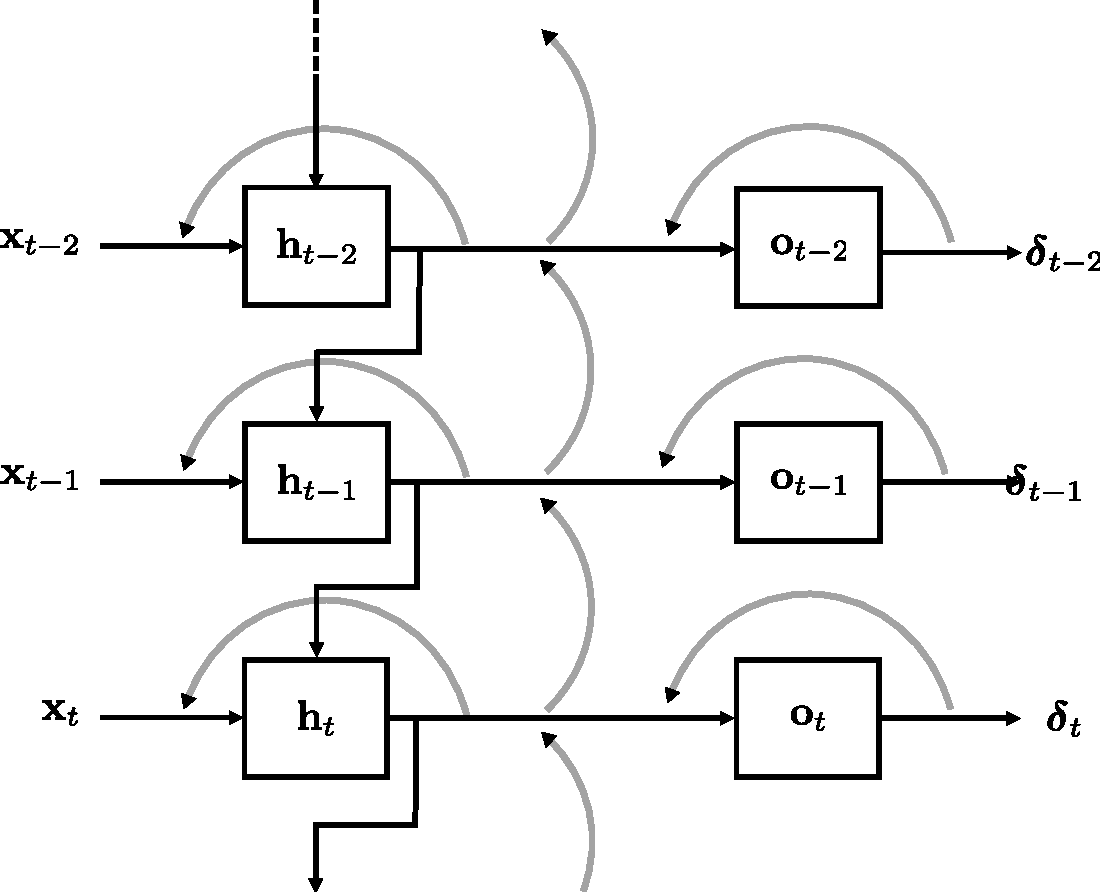
\includegraphics[scale=0.45]{Module 5 (RNN)/pics/smaller_rnn_unrolled_BP.pdf}
    \end{center}
\end{frame}

\end{document}